% sample.tex
\documentclass[9pt]{beamer}
\usepackage{}
\usepackage{pdfpages}
\usepackage{hyperref}
\usepackage[capitalise,nameinlink]{cleveref}
\hypersetup{colorlinks=true, linkcolor=blue, citecolor=blue, urlcolor=blue}
\usepackage{booktabs}
\definecolor{darkblue}{rgb}{0.0, 0.0, 0.55}
\usepackage{multicol}
\usepackage{xcolor}
\usepackage{pbox}
\usepackage{color}
\colorlet{linkequation}{blue}
\usepackage{bm, bbm}
\definecolor{forestgreen(web)}{rgb}{0.13, 0.55, 0.13}
\usepackage{float}
\usepackage{soul}
% \usepackage{hyperref}
% \usepackage[capitalise,nameinlink]{cleveref}
\usepackage[round]{natbib}
\usepackage{subfig}
% \captionsetup[subfigure]{labelformat=empty}  % Commented out as it's unused
\usepackage{algorithm,algorithmic}
\renewcommand{\algorithmicrequire}{\textbf{Input:}}
\renewcommand{\algorithmicensure}{\textbf{Output:}}
\usepackage{graphicx}
\usepackage{subcaption} 
\usepackage{mathtools}
\usepackage{multicol}
\usepackage{pgf,tikz}
\usepackage[round]{natbib}
\usepackage{makecell}
\usepackage{xeCJK}
\xeCJKsetup{CJKmath=false}


% \usepackage{fontspec}
% \usepackage{xeCJK}
% \xeCJKsetup{CJKmath=false}
% \setCJKmainfont{SimSun}
\bibliographystyle{plainnat}

\usetikzlibrary{arrows,shapes.arrows,shapes.geometric,shapes.multipart,fit,automata,decorations.pathmorphing,positioning}
\tikzset{
	%Define standard arrow tip
	>=stealth',
	%Define style for boxes
	true/.style={
		rectangle,
		draw=black, very thick,
		text width=6.5em,
		minimum height=2em,
		text centered,
		fill=gray, opacity = 0.5},
	punkt/.style={
		rectangle,
		rounded corners,
		draw=black, very thick,
		text width=6.5em,
		minimum height=2em,
		text centered},
	est/.style={
		circle,
		draw=black, very thick,
		text centered},
	shade/.style={
		circle,
		draw=black, very thick, fill=gray!50,
		text centered},
	weight/.style={
		circle,
		draw=black, very thick,
		text width=6.5em,
		minimum height=2em,
		text centered},
	% Define arrow style
	pil/.style={
		->,
		thick,
		shorten <=2pt,
		shorten >=2pt,},
	double/.style={
		<->,
		thick,
		shorten <=2pt,
		shorten >=2pt,},
	dash/.style={
		dashed,
		thick,
		shorten <=2pt,
		shorten >=2pt,},
	dashdouble/.style={
		<->,
		dashed,
		thick,
		shorten <=2pt,
		shorten >=2pt,}
}
%gets rid of footer
%will override 'frame number' instruction above
%comment out to revert to previous/default definitions
\setbeamertemplate{footline}{}
\usepackage{listings}
\definecolor{turquoise}{rgb}{0.19, 0.84, 0.78}

\definecolor{codegreen}{rgb}{0,0.6,0}
\definecolor{codegray}{rgb}{0.5,0.5,0.5}
\definecolor{codepurple}{rgb}{0.58,0,0.82}
\definecolor{backcolour}{rgb}{0.95,0.95,0.92}

\lstdefinestyle{mystyle}{
    backgroundcolor=\color{backcolour},    
    commentstyle=\color{codegreen},
    keywordstyle=\color{magenta},
    numberstyle=\tiny\color{codegray},
    stringstyle=\color{codepurple},
    basicstyle=\ttfamily\footnotesize,
    breakatwhitespace=false,         
    breaklines=true,                 
    captionpos=b,                    
    keepspaces=true,                 
    numbers=left,                    
    numbersep=5pt,                  
    showspaces=false,                
    showstringspaces=false,
    showtabs=false,                  
    tabsize=2
}

\lstset{style=mystyle}
\usepackage[most]{tcolorbox}
%\usetheme{default}
\usepackage{amsmath}
\usepackage{amsthm}
\usepackage{amsfonts}
\usepackage{amsopn}
\usepackage{scalerel}
\usepackage{cancel}
% Define argmin operator
\DeclareMathOperator*{\argmin}{arg\,min}

\newcommand\Wider[2][7.5em]{%
\makebox[\linewidth][c]{%
  \begin{minipage}{\dimexpr\textwidth+#1\relax}
  \raggedright#2
  \end{minipage}%
  }%
}
\newcommand\reallywidehat[1]{%
\begin{array}{c}
\stretchto{
  \scaleto{
    \scalerel*[\widthof{#1}]{\bigwedge}
    {\rule[-\textheight/2]{1ex}{\textheight}} %WIDTH-LIMITED BIG WEDGE
  }{1.25\textheight} % THIS STRETCHES THE WEDGE A LITTLE EXTRA WIDE
}{0.5ex}\\           % THIS SQUEEZES THE WEDGE TO 0.5ex HEIGHT
#1\\                 % THIS STACKS THE WEDGE ATOP THE ARGUMENT
\rule{-1ex}{0ex}
\end{array}
}
\usepackage{bbm}
% amssymb package, useful for mathematical symbols
\usepackage{amssymb}
\setbeamertemplate{theorems}[numbered]
\setbeamertemplate{lemma}[numbered]
\setbeamertemplate{corollary}[numbered]

\newcommand{\calW}{{\mathcal{W}}}
\def\m{\mathrm{m}}
\def\bbE{\mathbb{E}}
\def\bbP{\mathbb{P}}
\def\E{\mathsf{E}}
\def\Holder{\text{H\"{o}lder}}
\def\Pr{\mathsf{Pr}}
\def\EIF{\mathsf{EIF}}
\def\NIF{\mathsf{NIF}}
\def\bias{\texttt{bias}}
\def\var{\texttt{var}}
\def\cov{\texttt{cov}}

\def\tilde{\widetilde}
\def\P{\mathsf{P}}
\def\calP{\mathcal{P}}
\def\d{\mathrm{d}}
\def\calG{\mathcal{G}}
\def\pa{\mathsf{pa}}
\def\ch{\mathsf{ch}}
\def\an{\mathsf{an}}
\def\de{\mathsf{de}}
\def\bV{\bm{V}}
\def\bv{\bm{v}}
\def\be{\bm{e}}
\def\var{\mathsf{var}}
\def\cov{\mathsf{cov}}
\def\df{\mathrm{df}}
\def\init{\mathrm{init}}
\def\t{\mathrm{t}}
\def\calA{\mathcal{A}}

\DeclareRobustCommand{\stred}[1]{{\sethlcolor{cyan}\st{#1}}}
\setbeamercovered{transparent}
\setbeamertemplate{theorems}[numbered]
\makeatletter
\def\th@mystyle{%
    \normalfont % body font
    \setbeamercolor{block title example}{bg=gray,fg=white}
    \setbeamercolor{block body example}{bg=white,fg=black}
    \def\inserttheoremblockenv{exampleblock}
  }
\makeatother
\theoremstyle{mystyle}
\definecolor{dblue}{named}{fg}
\newtheorem{mytheorem}{Theorem}
\newtheorem{mycorollary}{Corollary}
\newtheorem{myprop}{Proposition}
\newtheorem{mylemma}{Lemma}
\newtheorem{myfact}{Fact}
\newtheorem{mydefn}{Definition}
\newtheorem{myeg}{Example}
\newtheorem{myremark}{Remark}
\newtheorem{myqn}{Qn}
\definecolor{ForestGreen}{RGB}{34,139,34}

\makeatletter
\def\th@mystyletwo{%
    \normalfont % body font
    % \setbeamercolor{block title example}{bg=orange,fg=white}
    \setbeamercolor{block body example}{bg=orange!20,fg=black}
    \def\inserttheoremblockenv{exampleblock}
  }
\makeatother
\theoremstyle{mystyletwo}
\newtheorem*{myblock}{}
\usepackage{tikzsymbols}
\usepackage{textcomp}

\definecolor{greyone}{RGB}{77,77,77}
\setbeamercolor{palette quaternary}{fg=white}
\setbeamercolor{titlelike}{parent=palette quaternary}
% \usepackage{enumitem}
\setbeamercolor{title}{fg=black}
\setbeamerfont{title}{series=\bf, size=\Large}
\setbeamercolor{frametitle}{fg=brown!150}

\setbeamerfont{frametitle}{size=\Large}
\setbeamertemplate{itemize/enumerate body begin}{\normalsize}
\setbeamertemplate{itemize/enumerate subbody begin}{\normalsize}

%gets rid of bottom navigation bars
%\setbeamertemplate{footline}[frame number]{}

\setbeamertemplate{frametitle}[default][center]

%gets rid of bottom navigation symbols
\setbeamertemplate{navigation symbols}{}

\newcommand\independent{\protect\mathpalette{\protect\independenT}{\perp}}
\def\independenT#1#2{\mathrel{\rlap{$#1#2$}\mkern2mu{#1#2}}}

%\expandafter\def\expandafter\insertshorttitle\expandafter{%
%  \insertshorttitle\hfill%
%  \insertframenumber\,/\,\inserttotalframenumber}
\addtobeamertemplate{navigation symbols}{}{ \hspace{1em}    \usebeamerfont{footline}%
    \large\insertframenumber / \inserttotalframenumber }

\def\calF{\mathcal{F}}
\def\Holder{H\"{o}lder}
\def\bbE{\mathbb{E}}
\def\bE{\mathbf{E}}
\def\bZ{\mathbf{Z}}
\def\bz{\mathbf{z}}
\def\bX{\mathbf{X}}
\def\bx{\mathbf{x}}
\def\bY{\mathbf{Y}}
\def\y{\mathrm{y}}
\def\a{\mathrm{a}}
\def\bbP{\mathbb{P}}
\def\Infl{\mathsf{IF}}
\def\diff{\mathrm{d}}
\def\a{\mathrm{a}}
\def\b{\mathrm{b}}
\def\hata{{\color{blue}\hat{\a}}}
\def\hatb{{\color{blue}\hat{\b}}}
\def\N{\mathrm{N}}
\def\bmu{\bm{\mu}}
\def\bSigma{\bm{\Sigma}}
\def\bbeta{\bm{\beta}}
\def\balpha{\bm{\alpha}}
\def\db{\mathsf{db}}
\def\reg{\mathsf{reg}}
\def\bI{\mathbf{I}}

\def\bbX{\mathbb{X}}

% Custom block width commands
\newcommand{\fullwidth}{\linewidth}
\newcommand{\halfwidth}{0.49\linewidth}
\newcommand{\thirdwidth}{0.32\linewidth}
\newcommand{\unknowna}[1]{\textcolor{teal!70!black}{#1}}
\newcommand{\unknownb}[1]{\textcolor{orange!80!black}{#1}}
\newcommand{\unknownc}[1]{\textcolor{violet!70!black}{#1}}
\newcommand{\unknownd}[1]{\textcolor{gray!60!black}{#1}}
\newcommand{\unknowne}[1]{\textcolor{green!60!black}{#1}}
\newcommand{\unknownh}[1]{\textcolor{blue!65!black}{#1}}



\def\f{\mathrm{f}}

\def\bbE{\mathbb{E}}
\def\bbP{\mathbb{P}}
\def\E{\mathsf{E}}
\def\Holder{\text{H\"{o}lder}}
\def\Pr{\mathsf{Pr}}
\def\EIF{\mathsf{EIF}}
\def\NIF{\mathsf{NIF}}
\def\bias{\texttt{bias}}
\def\var{\texttt{var}}
\def\cov{\texttt{cov}}
\def\hat{\widehat}
\def\tilde{\widetilde}
\def\P{\mathsf{P}}
\def\calP{\mathcal{P}}
\def\d{\mathrm{d}}
\def\calG{\mathcal{G}}
\def\pa{\mathsf{pa}}
\def\ch{\mathsf{ch}}
\def\an{\mathsf{an}}
\def\de{\mathsf{de}}
\def\bV{\bm{V}}
\def\bv{\bm{v}}
\def\be{\bm{e}}
\def\bU{\bm{U}}
\def\var{\mathsf{var}}
\def\cov{\mathsf{cov}}
\def\df{\mathrm{df}}
\def\init{\mathrm{init}}
\def\t{\mathrm{t}}
\newcommand{\calX}{{\mathcal{X}}}
\newcommand{\bbU}{{\mathbb{U}}}
\newcommand{\bbV}{{\mathbb{V}}}

\def\calF{\mathcal{F}}
\def\Holder{H\"{o}lder}
\def\bbE{\mathbb{E}}
\def\bE{\mathbf{E}}
\def\bZ{\mathbf{Z}}
\def\bX{\mathbf{X}}
\def\bx{\mathbf{x}}
\def\bY{\mathbf{Y}}
\def\A{\mathrm{A}}
\def\Y{\mathrm{Y}}
\def\y{\mathrm{y}}
\def\a{\mathrm{a}}
\def\bbP{\mathbb{P}}
\def\Infl{\mathsf{IF}}
\def\diff{\mathrm{d}}
\def\a{\mathrm{a}}
\def\b{\mathrm{b}}
\def\hata{{\color{blue}\hat{\a}}}
\def\hatb{{\color{blue}\hat{\b}}}
\def\N{\mathrm{N}}

\def\bmu{\bm{\mu}}

\def\bbeta{\bm{\beta}}
\def\balpha{\bm{\alpha}}
\def\db{\mathsf{db}}
\def\reg{\mathsf{reg}}
\def\bI{\mathbf{I}}

\def\({\left(}
\def\){\right)}
\def\[{\left[}
\def\]{\right]}
\def\bbR{\mathbb{R}}

\def\f{\mathrm{f}}
\def\({\left(}
\def\){\right)}
\def\[{\left[}
\def\]{\right]}
\def\bbR{\mathbb{R}}
    
\tcbset{
  mytheoremstyle/.style={
    colback=white,
    colframe=blue!60!black,
    fonttitle=\bfseries,
    coltitle=black,
    title={Questions},
    sharp corners,
    boxrule=0.8pt,
    left=6pt, right=6pt, top=6pt, bottom=6pt,
  }
}
\tcbset{
  myposterstyle/.style={
    colback=white,
    colframe=blue!80!black,
    coltitle=white,
    colbacktitle=blue!80!black,
    fonttitle=\bfseries,
    boxrule=1pt,
    sharp corners,
    enhanced,
    left=6pt, right=6pt, top=6pt, bottom=6pt,
    titlerule=0mm,
    toptitle=1mm,
    bottomtitle=1mm
  }
}

% user-defined commands
% user-defined macros
\newcommand{\pdfu}{\texorpdfstring{$U$}{U}}
\newcommand{\pdfv}{\texorpdfstring{$V$}{V}}
\newcommand{\libref}[2]{\href{#2}{\texttt{#1}}}

\newcommand{\mobius}{M\"obius}

\newcommand{\numpy}{\libref{numpy}{https://numpy.org/}}
\newcommand{\torch}{\libref{pytorch}{https://pytorch.org/}}

% simplified command
\newcommand{\wt}{\overline}
\newcommand{\diag}{\mathsf{Diag}}
\newcommand{\diagp}[1]{\diag(#1)}
\newcommand{\sPi}{\pi}
\newcommand{\sper}{\sigma}

% HOIF
\newcommand{\IF}{\mathbb{IF}}
\newcommand{\BD}{\mathbb{BD}}
\newcommand{\factorial}[1]{#1\mathpunct{!}}

% stats notations
\newcommand{\uset}{\calU}
\newcommand{\usetnm}[2]{\uset\left(#1,#2\right)}
\newcommand{\vset}{\calV}
\newcommand{\vsetp}[2]{\vset(#1,#2)}

\newcommand{\ustat}{\mathbb{U}}
\newcommand{\vstat}{\mathbb{V}}
\newcommand{\ustatp}[2]{\ustat(#1,#2)}
\newcommand{\vstatp}[2]{\vstat(#1,#2)}

% set notations
\newcommand{\samplespace}{\bbX}
\newcommand{\takesetp}[1]{\mathsf{set}[#1]}
\newcommand{\cartesianprod}{\bigotimes}

% combinatoric notations
\newcommand{\perm}[1]{\mathsf{Perm}(#1)}
\newcommand{\partition}{\Pi}

\newcommand{\partitionp}[1]{\partition_{#1}}
\newcommand{\finest}{\mathsf{Fin}}
\newcommand{\finestp}[1]{\finest[#1]}
\newcommand{\coarsest}{\mathsf{Coa}}
\newcommand{\coarsestp}[1]{\coarsest[#1]}
\newcommand{\cover}{\mathcal{C}}
\newcommand{\stirling}{\calS}
\newcommand{\stirlingp}[2]{\stirling(#1,#2)}

% tensor notations
\newcommand{\ndim}{\mathsf{ndim}}
\newcommand{\ndimp}[1]{\ndim(#1)}
\newcommand{\rank}{\mathrm{rank}}
% \newcommand{\dim}{\mathrm{dim}}
\newcommand{\dimp}[2]{\dim[#1](#2)}
\newcommand{\indexset}{\mathsf{Indices}}
\newcommand{\teq}{\overset{\mathrm{t.e.}}{=}}
\newcommand{\canonicalform}{\mathsf{canonical}}
\newcommand{\tensorcontraction}{\mathsf{Contraction}}

% partial order in partition
\newcommand{\pleq}{\preceq}
\newcommand{\pgeq}{\succeq}
\newcommand{\pless}{\prec}
\newcommand{\pgreater}{\succ}

% Graph notations
\newcommand{\degp}[2]{\deg_{#2}(#1)}
\newcommand{\vertices}[0]{V}
\newcommand{\verticesp}[1]{V(#1)}
\newcommand{\edges}[0]{E}
\newcommand{\edgesp}[1]{E(#1)}
\newcommand{\neighborvg}[2]{N_{#2}(#1)}

\newcommand{\treewidth}{\mathsf{tw}}
\newcommand{\treewidthp}[1]{\mathsf{tw}(#1)}
\newcommand{\quotientgraphp}[1]{\mathcal{Q}(#1)}
\newcommand{\graphset}{\mathcal{G}^{*}}
\newcommand{\graphsetne}[2]{\mathcal{G}_{#1,#2}^{*}}

\newcommand{\degeneracy}{D}
\newcommand{\degeneracyg}[1]{\degeneracy(#1)}
\newcommand{\completegraphp}[1]{\mathrm{K}_{#1}}
\newcommand{\graphtype}[1]{G_{#1}}
\newcommand{\motifrg}[2]{\mathsf{C}(#1,#2)}
% Oh-notaions
\newcommand{\greater}{\Omega}
\newcommand{\less}{O}
\newcommand{\muchgreater}{\omega}
\newcommand{\muchless}{o}
\newcommand{\appequal}{\Theta}

% operators
\newcommand{\eliminatevg}[2]{\mathsf{elim}_{#1}(#2)}


\def\eps{\epsilon}
\def\veps{\varepsilon}
\def\mse{\mathsf{mse}}

% code libs 
\def\package{\libref{u-stats}{https://github.com/Amedar-Asterisk/U-Statistics-python}}

\newcommand{\numpyeinsum}{\libref{numpy.einsum}{https://numpy.org/doc/2.1/reference/generated/numpy.einsum.html}}

\newcommand{\torcheinsum}{\libref{pytorch.einsum}{https://pytorch.org/docs/stable/generated/torch.einsum.html}}
\newcommand{\opteinsum}{\libref{opt-einsum}{https://dgasmith.github.io/opt_einsum/}}
\newcommand{\igraph}{\libref{igraph}{https://igraph.org/}}
\graphicspath{{Figures_slides/}}

\title{On Computing and the Complexity of Computing Higher-Order U-Statistics, Exactly}
\date{2025年9月20日}
\author[陈星宇]{陈星宇\\
上海交通大学 \\
数学科学学院 \\
Email: \texttt{xingyuchen0714@sjtu.edu.cn} \\
}

\institute{中国现场统计研究会统计交叉科学研究分会 \\
全国工业统计学教学研究会民族统计与数据科学分会2025联合年会}



\begin{document}
\begin{frame}
    \maketitle
\end{frame}

\begin{frame}
  \frametitle{Coauthors}
  \centering
  \begin{minipage}[b]{0.4\textwidth}
    \centering
    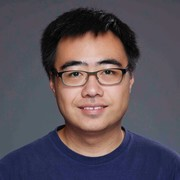
\includegraphics[height=4cm]{Figures_slides/Lin_Liu.png}
    刘林, 上海交通大学
  \end{minipage}
  \hfill
  \begin{minipage}[b]{0.4\textwidth}
    \centering
    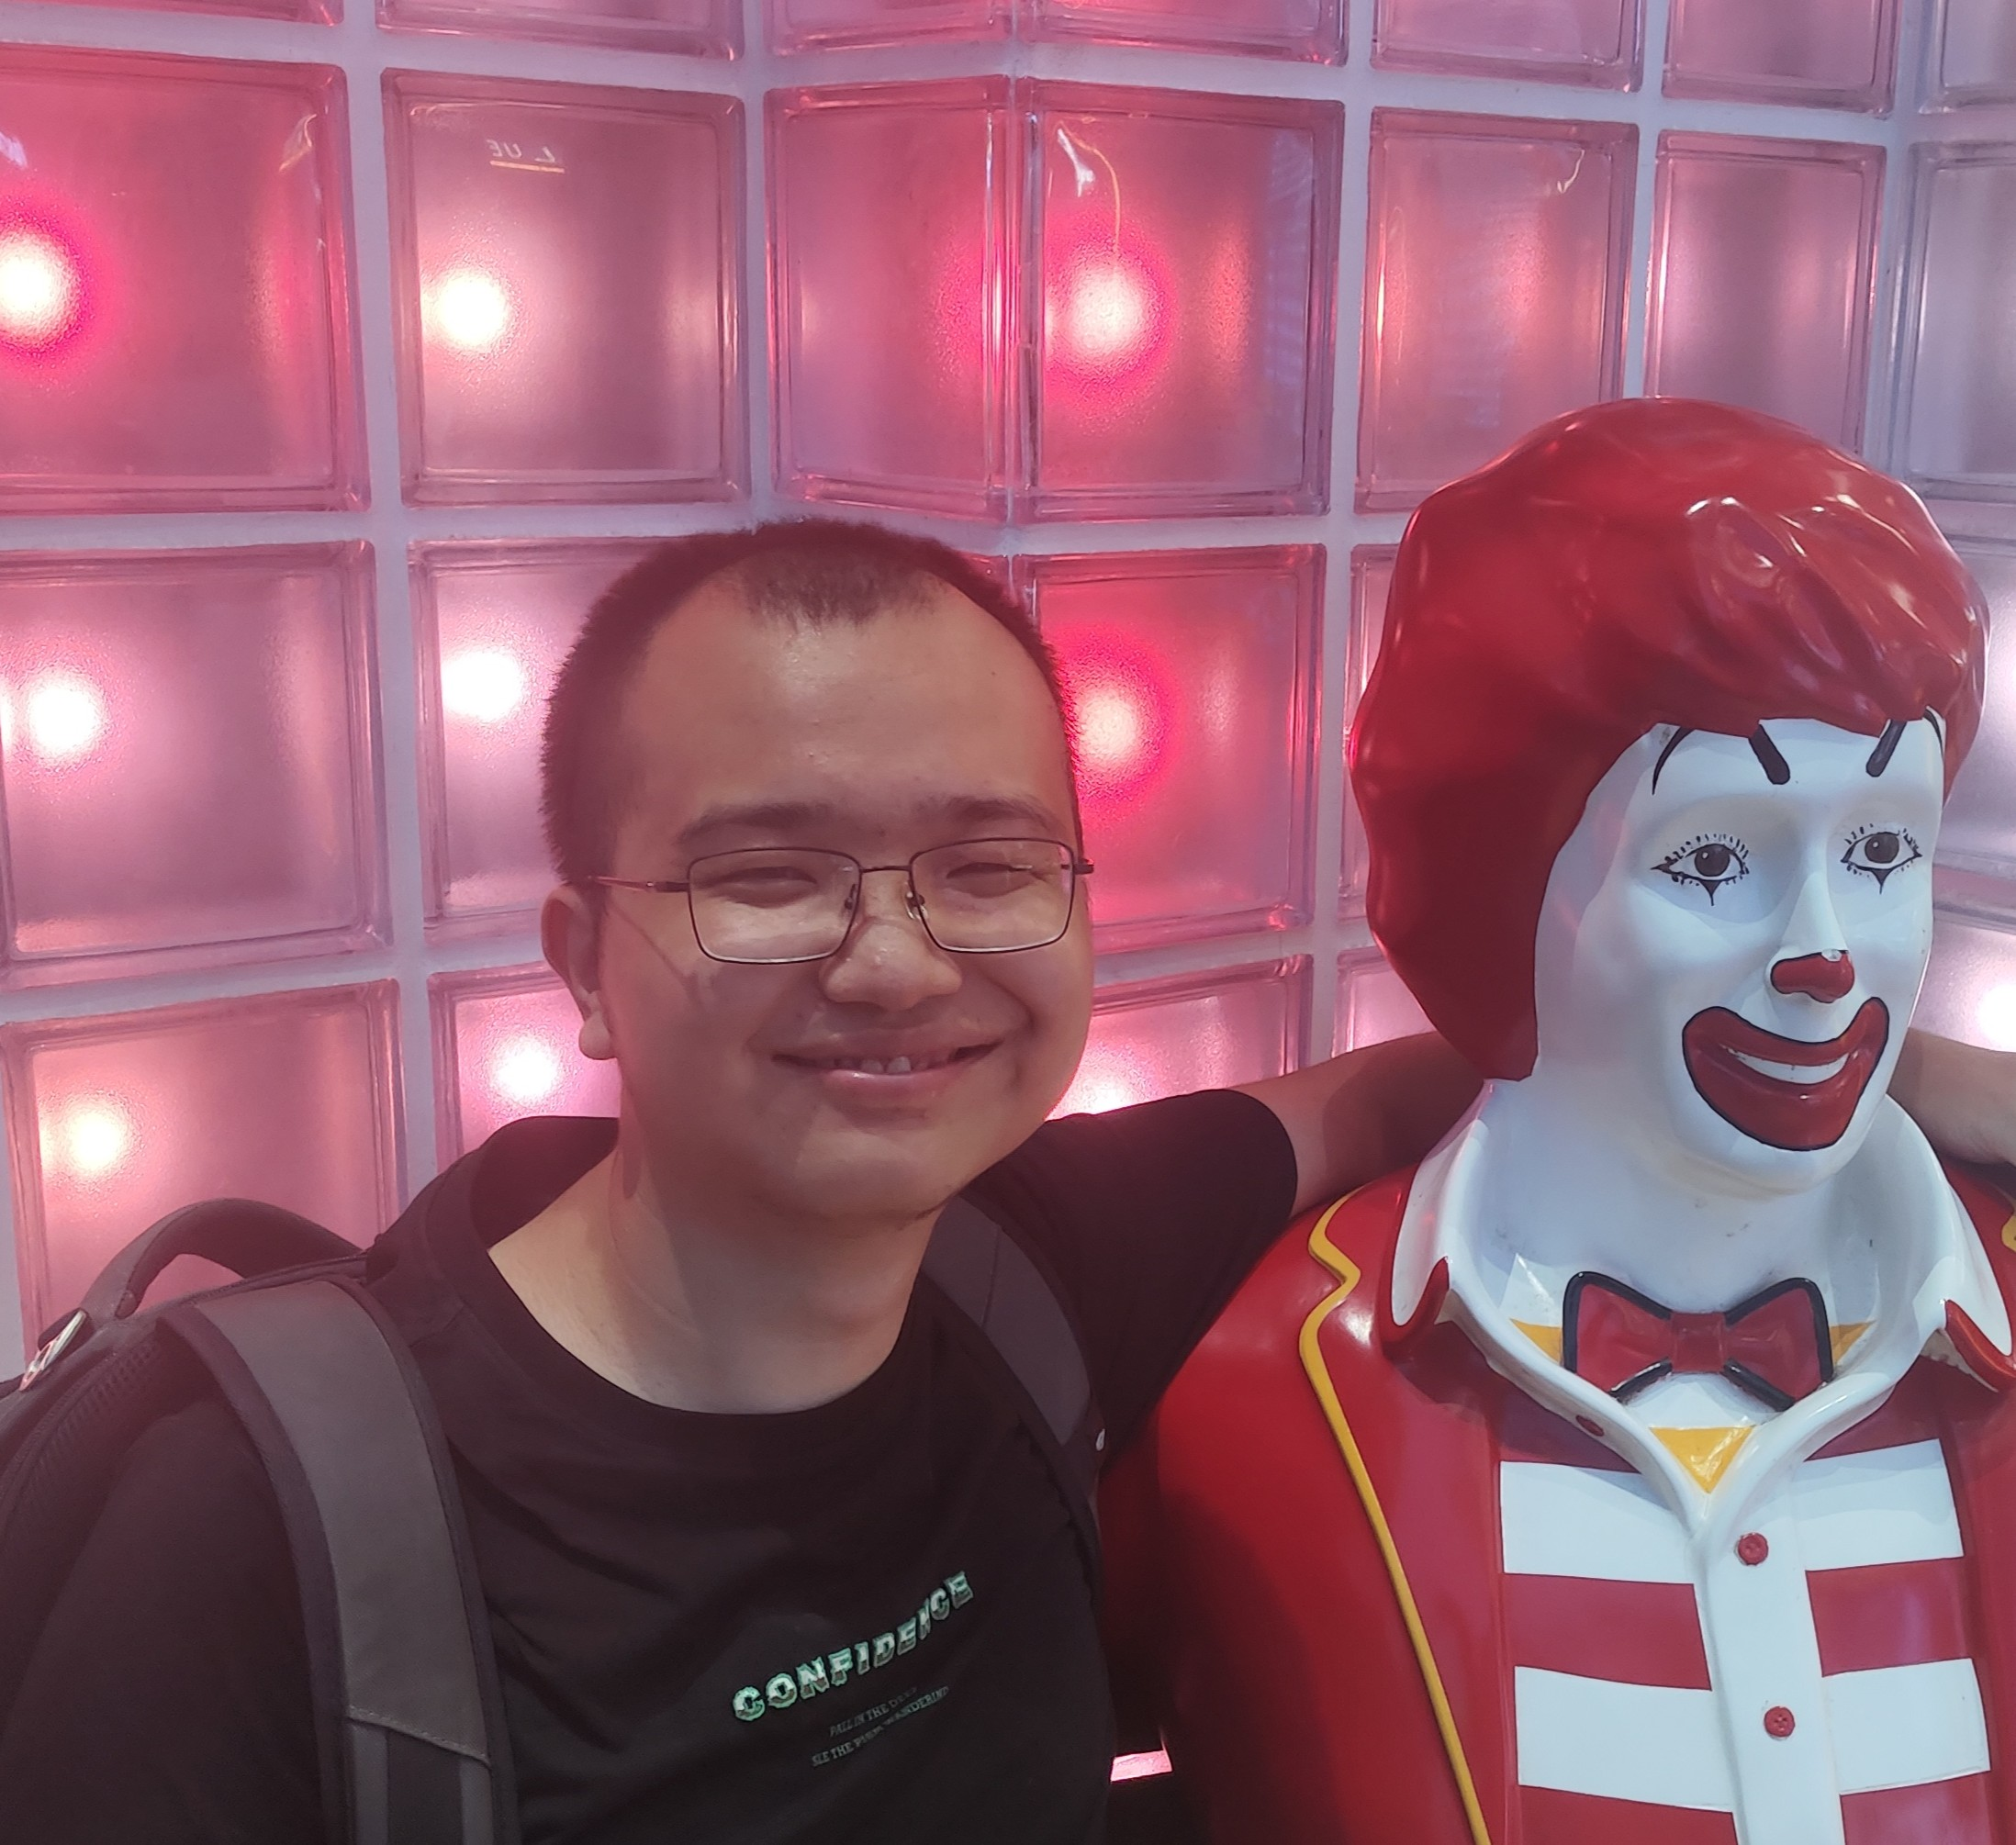
\includegraphics[height=4cm]{Figures_slides/Ruiqi_Zhang.jpg}
    张瑞琦, 华东师范大学
  \end{minipage}
\end{frame}


% \begin{frame}\frametitle{Outline}
%     \tableofcontents[currentsection, sectionstyle=show, subsectionstyle=show]
% \end{frame}

\section{On Computing U-Statistics}
\begin{frame}
    \frametitle{Outline}
    \tableofcontents[currentsection, sectionstyle=show/shaded, subsectionstyle=show/shaded/shaded]
\end{frame}
\begin{frame}
    \frametitle{U/V-Statistics}
    U-statistics are generally used to construct unbiased estimators of population parameters.
    \begin{itemize}
        \item Given a kernel $h(x_1, \ldots, x_m): \calX^m \to \bbR$ and a sequence of samples $X_1, \ldots, X_n$. 
        \item The U-statistic takes the form
              \begin{align*}
                  \mathbb{U}_{n,m}[h] = \cancel{\frac{n!}{(n-m)!}} \sum_{1 \le i_1 \neq i_2 \neq \cdots \neq i_m \le n} h(X_{i_1}, \ldots, X_{i_m}).
              \end{align*}
        \item The V-statistic takes the form
              \begin{align*}
                  \mathbb{V}_{n,m}[h] = \cancel{\frac{1}{n^m}} \sum_{1 \le i_1,i_2,\cdots,i_m \le n} h(X_{i_1}, \ldots, X_{i_m}).
              \end{align*}
        \item There is a linear relationship between $U$-statistics and $V$-statistics
        \begin{align*}
            \mathbb{U} = \sum \mathbb{V}, \mathbb{V} = \sum \mathbb{U}.
        \end{align*}
        Thus, if $\mathbb{V}$ can be computed efficiently, then so can $\mathbb{U}$, and vice versa.
    \end{itemize}
\end{frame}

\begin{frame}
\frametitle{The answer: V-statistics can be computed by \texttt{Einsum}}

    \begin{itemize}
        \item \texttt{Einsum} can be used to compute the V-statistic efficiently.
              \begin{itemize}
                    \item The \texttt{Einsum} operation mainly performs \textbf{unconstrained summation} over selected indices of input tensors.
                  \item Can call \numpyeinsum{} or \torcheinsum{} in practice.
                  \item \torch{} provides parallel computing on CPU and GPU.
              \end{itemize}
        \item Examples:
        \begin{columns}
            \begin{column}{0.8\textwidth}
                \centering
                              
                \texttt{\large Einsum('ij,jk->ik', A, B)}
                
                \large $  \sum_j A_{ij} B_{jk} = D_{ik}$
                        
                \vspace{0.4cm}
        
                
                \texttt{ \large Einsum('ijk->i', X)}
                
                \large$ \sum_{j,k} X_{ijk} = D_i $
                
                \vspace{0.4cm}
                
                \texttt{ \large Einsum('ij,jk,kl->', A, B, C)}
                
                \large $  \sum_{i,j,k} A_{ij} \, B_{jk} \, C_{kl} = D$
                        
                \vspace{0.4cm}
            \end{column}
        \end{columns}

\item Then what's the exact formula of the $ \mathbb{U} = \sum \mathbb{V}$?

    \end{itemize}

\end{frame}


\begin{frame}
    \frametitle{Decomposition of U-statistics to V-statistics}
    \begin{itemize}
        \item The exact formula  can be written as following:
        \item The proof will use the \textbf{M\"obius inversion} technique.
              \begin{mylemma}[C., Zhang, Liu, 25]
                  \label{lem:decomp_u_to_v}
                  Let $\bbX$ be a non-empty set and $h: \bbX^{m} \rightarrow \bbR$ be a kernel function. Then for any $\bm{X} \in \bbX^n: n \geq m$,
                  \begin{align*}
                      \ustat[h] = \sum_{\sPi \in \partitionp{m}}
                      \mu_\sPi \vstat[\sPi](h),
                  \end{align*}
                  where
                  \begin{align*}
                      \mu_\sPi = (-1)^{(m-|\sPi|)} \prod_{C \in \sPi} (|C| - 1)!,
                  \end{align*}
                  and $\partitionp{m}$ denotes all partition of set $\{1,2,\cdots,m\}.$
              \end{mylemma}

    \end{itemize}
\end{frame}

\begin{frame}
    \frametitle{Decomposition of U-statistics to V-statistics}
    \begin{itemize}
        \item The definition of $\vstat[\sPi](h)$ is as following:
     \begin{align*}
     \pi = \{\{1\},\{2\},\{3\}\},\quad & \mathbb{V}[\pi](h) = \sum_{i_1,i_2,i_3} h(X_{i_1},X_{i_2},X_{i_3}), \quad \mu_{\pi} = +1,\\
     \pi = \{\{1,2\},\{3\}\},\quad & \mathbb{V}[\pi](h) = \sum_{i_1=i_2,i_3} h(X_{i_1},X_{i_2},X_{i_3}), \quad \mu_{\pi} = -1, \\
     \pi = \{\{1,3\},\{2\}\},\quad & \mathbb{V}[\pi](h) = \sum_{i_1=i_3,i_2} h(X_{i_1},X_{i_2},X_{i_3}), \quad \mu_{\pi} = -1, \\
     \pi = \{\{2,3\},\{1\}\},\quad & \mathbb{V}[\pi](h) = \sum_{i_2=i_3,i_1} h(X_{i_1},X_{i_2},X_{i_3}), \quad \mu_{\pi} = -1, \\
     \pi = \{\{1,2,3\}\},\quad & \mathbb{V}[\pi](h) = \sum_{i_1=i_2=i_3} h(X_{i_1},X_{i_2},X_{i_3}),\quad \mu_{\pi} = +2.
    \end{align*}

    \item For $m = 3$:
    \begin{align*}
        \mathbb{U}[h] & = \sum_{i_1 \neq i_2 \neq i_3} h(X_{i_1},X_{i_2},X_{i_3}) \\
 & = \Big(\sum_{i_1,i_2,i_3} - \sum_{(i_1=i_2), i_3 } - \sum_{(i_1=i_3), i_2 } - \sum_{(i_2=i_3), i_1 } + 2 \sum_{i_1=i_2=i_3}\Big) h(X_{i_1},X_{i_2},X_{i_3}).
    \end{align*}
    \end{itemize}
\end{frame}

\begin{frame}
\frametitle{Algorithm Framework }

\begin{center}
\begin{minipage}{1.0\textwidth}

\begin{tcolorbox}[colback=white,colframe=blue!50!black,title=Basic Algorithm Framework]
\begin{flushleft}
\textbf{Input:} Kernel function $h$, data samples $X_1,\ldots,X_n$, order $m$ \\
\textbf{Output:} U-statistic $\ustat[h]$
\end{flushleft}

\vspace{0.2cm}
\begin{enumerate}
    \item Initialize $\ustat[h] \gets 0$
    \item For each partition $\pi \in \partitionp{m}$:
    \begin{enumerate}
        \item Compute coefficient $\mu_{\pi}$
        \item Compute V-statistic $\vstat[\pi](h)$ via \texttt{Einsum}
        \item $\ustat[h] \gets \ustat[h] + \mu_{\pi} \cdot \vstat[\pi](h)$
    \end{enumerate}
    \item Return $\ustat[h]$
\end{enumerate}
\end{tcolorbox}


\end{minipage}
\end{center}

\end{frame}


% \begin{frame}
%     \frametitle{Our New Package \package{} for Computing U-Statistics}
%     \begin{itemize}
%         \item Github Link:  \url{https://github.com/Amedar-Asterisk/U-Statistics-python}
%         \item Some instructions can also be found in the \texttt{README.md} file of the repository.
%     \end{itemize}
%     \begin{figure}
%         \centering
%         
\includegraphics[width=0.5\linewidth]{github_QR.png}
%         \caption*{\package{} Github link}
%     \end{figure}
% \end{frame}

\section{On Complexity of Computing  U-Statistics}
\begin{frame}
    \frametitle{Outline}
    \tableofcontents[currentsection, sectionstyle=show/shaded, subsectionstyle=show/shaded/shaded]
\end{frame}

\begin{frame}
    \frametitle{New Questions Arising in Computing U-Statistics}
    The following questions naturally arise:
    
    \begin{block}{Question 1}
        How to characterize the computational complexity theoretically?
    \end{block}
    \begin{itemize}
        \item The naive nested-loop approach requires {\color{red}$O(n^m)$}.
        \item Can the new algorithm compute U-statistics in {\color{red}substantially less than $O(n^m)$} time?
    \end{itemize}

\begin{block}{Question 2}
    The number of all set partitions $\pi \in \partitionp{m}$ is large, given by the \textbf{Bell number} $B_m$. 
    Do we really need so many terms?
    \begin{itemize}
        \item $B_m$ increases \textbf{super-exponentially} with $m$.
        \item For example:
        \begin{align*}
        B_6 &= 203, \quad B_7 = 877, \quad B_8 = 4140, \\ B_9 &= 21147, \quad B_{10} = 115975.
        \end{align*}
    \end{itemize}
\end{block}


    \vspace{0.2cm}
    \centering
    Both answers will strongly depend on the \textbf{structure of the kernel function $h$}.
\end{frame}



\begin{frame}
    \frametitle{Example 1: U-Statistics in Causal Inference: HOIFs}
    \begin{itemize}
        \item Higher-order influence functions (HOIFs) \citep{robins2008higher, robins2016technical} are rate-optimal estimators for many causal parameters. 
        % under various structural assumptions (smoothness, structure-agnostic, …)
        \item HOIFs are high order U-statistics, whose order can be up to $m \sim \sqrt{\log n}$.
        \item For example, HOIF of the treatment-specific mean is the combination of functions like
              
    \begin{tcolorbox}[colframe=blue!70!black, colback=blue!5, 
                  boxrule=1.0pt, arc=1mm, 
                  enhanced, breakable]
    \begin{align*}
      &  h^{\mathsf{HOIF}}_m(X_{1}, \ldots, X_{m}) \\
      & = [a_{{1}} \phi (Z_{{1}})^{\top} \phi(Z_{2})]  [\phi (Z_{{2}})^{\top} \phi(Z_{3})] \cdots [\phi(Z_{{m-1}})^\top \phi(Z_{m})b_{m}] \\
      & = f_1(X_{1},X_{2})  f_2(X_{2},X_{3}) \cdots f_{m-1}(X_{m-1},X_{m})
    \end{align*}
    \end{tcolorbox}

    \item For Question 1, given the $n \times n$ matrices $A^{(k)}_{ij} = f_k(X_i, X_j)$ for $k = 1, \cdots, m-1$:
    \begin{equation*}
    \begin{split}
    \mathrm{Complexity}(\mathbb{U}_{n,m}(h^{\mathsf{HOIF}}_m)) = \left\{ \begin{array}{ll}
    O(n^2), & m \in \{2, 3\}, \\
    O(n^3), & m \in \{4, 5, 6, 7\}, \\
    O(n^4), & m \in \{8, 9, 10\}, \\
    O(n^5), & m \in \{11, 12\}.
    \end{array} \right.
    \end{split}
    \end{equation*}
        
    \item For Question 2, some terms will be canceled.
    
    \end{itemize}

\end{frame}

\begin{frame}
    \frametitle{Example 2: Dependence Measures}
    \begin{itemize}
        \item High-order U-statistics are also used to estimate dependence measures, such as Distance Covariance ($\mathsf{dCov}^2$) \citep{szekely2007measuring}.
        \item $\mathsf{dCov}^2$ can be represented as a 4-th order U-statistic \citep{yao2018testing}:
            \begin{tcolorbox}[colframe=blue!70!black, colback=blue!5, 
                  boxrule=1.0pt, arc=1mm, 
                  enhanced, breakable]
              \begin{align*}
                  \mathsf{dCov}^2(X, Y) = \frac{(n-4)!}{n!} \sum_{i \neq j \neq q \neq r}
                  a_{ij}b_{qr} + a_{ij}b_{ij} - a_{ij}b_{iq} - a_{ij}b_{jr}
              \end{align*}
               
              \end{tcolorbox}
              where $a_{ij} = \|X_i-X_j\|_2$ and $b_{ij} = \|Y_i-Y_j\|_2$.
        \item it can be decomposed to $3$ kernel function:


            \item For Question 1, given the $n \times n$ matrices $a_{ij},b_{ij}$:
            \begin{equation*}
            \mathrm{Complexity} (\mathsf{ dCov}^2(X Y) ) = O(n^2). 
            \end{equation*}
                
            \item For Question 2: Many terms will be canceled. 
            \end{itemize}
\end{frame}


\begin{frame}
\frametitle{Example 3: Motif Counts}
\begin{itemize}
    \item Motif counts refer to the number of occurrences of small subgraphs (motifs) in a random graph. 
    \item They can be used to test certain properties of the underlying random graphon \citep{chatterjee2024higher}.
    \item The motif counts can also be written as a form similar to U-statistics. 
    \item 3-node motifs,
        \begin{figure}
          \centering
          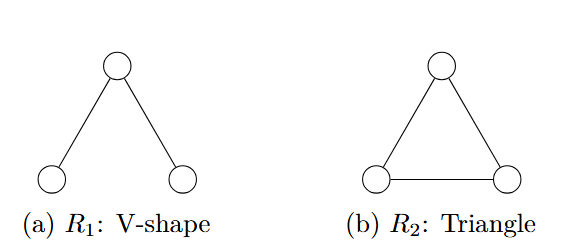
\includegraphics[width=0.5\linewidth]{motif3.jpg}
          \caption*{3-node motifs in a random graph}
          \label{fig:motif3}
      \end{figure}
\end{itemize}
\end{frame}

\begin{frame}
\frametitle{Example 3: Motif Counts}
\begin{itemize}
    \item 4-node motifs, 
        \begin{figure}
          \centering
          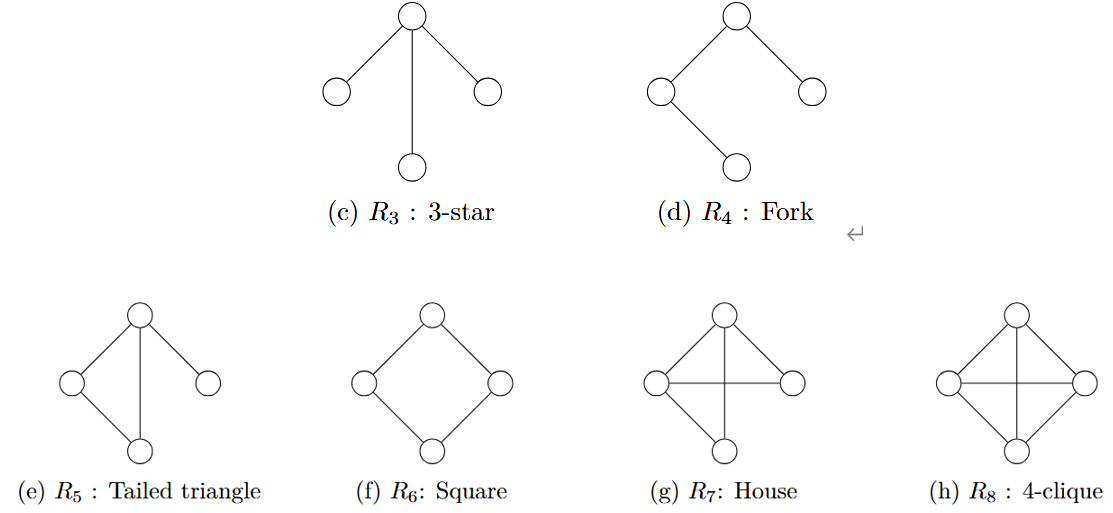
\includegraphics[width=0.9\linewidth]{motif4.jpg}
          \caption*{4-node motifs in a random graph}
          \label{fig:motif4}
        \end{figure}
\end{itemize}
\end{frame}

\begin{frame}
\frametitle{Example 3: Motif Counts}
\begin{itemize}

        \item For example :
            \begin{tcolorbox}
            [colframe=blue!70!black, colback=blue!5, 
                  boxrule=1.0pt, arc=1mm, 
                  enhanced, breakable]
                  \begin{itemize}
                      \item V-shape
                       \begin{align*}
                C(R_1) = \frac{1}{2} \sum_{ i_1 \neq i_2 \neq i_3}  A_{i_1 i_2} A_{i_2 i_3}  B_{i_3 i_1}
        \end{align*}
              \item Triangle:
        \begin{align*}
                C(R_2) = \frac{1}{6} \sum_{ i_1 \neq i_2 \neq i_3}  A_{i_1 i_2} A_{i_2 i_3}  A_{i_3 i_1}
        \end{align*}
             \item $A$ is the adjacency matrix of the graph and $ B = 1 - A$.
                  \end{itemize}
         \end{tcolorbox}
         \item  For Question 1, given adjacency matrix $A$, the complexity is still $O(n^m)$ for $m$-motif.
         \item For Question 2,  {\color{red} only $1$ term} is needed.
\end{itemize}
\begin{figure}
          \centering
          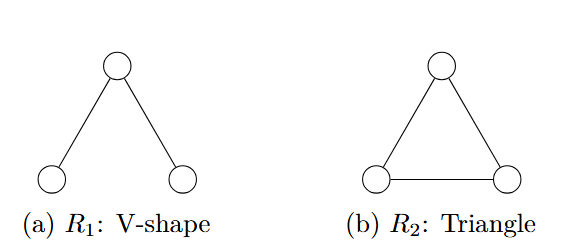
\includegraphics[width=0.4\linewidth]{motif3.jpg}
\end{figure}
\end{frame}

% \begin{frame}
% \frametitle{More Examples}
% \begin{itemize}
%     \item \cite{} used U-statistics to
%     \item \cite{} used U-statistics to
% \end{itemize}
% \end{frame}


\begin{frame}
    \frametitle{Key Assumption: Multiplicative-Decomposable}
    The key of answering the above questions is the \textbf{multiplicative-decomposition} of kernels.
    \begin{itemize}
        \item We observed that many kernels of U-statistics is product of some functions with less arguments.
        \item Let's give a notation to capture this structure, it mimics the \texttt{Einsum} notation "ij,jk -> ".
        \item For $h^{\mathsf{HOIF}}_3(\bm{X}) = f_1(X_1,X_2) f_2(X_2,X_3) $:
        \begin{align*}
           \calA^{\mathsf{HOIF}}_3 = ((1,2),(2,3)), T^{(k)}_{ij} = f_k(X_1,X_2), k =1,2.
        \end{align*}

        \pause
        
        \item For a part of $\mathsf{dCov}^2(X, Y)$: $ \frac{(n-4)!}{n!} \sum_{i \neq j \neq q \neq r}
                  a_{ij}b_{qr}$
        \begin{align*}
            \calA^{\mathsf{dCov},1} = ((1,2),(3,4)), T^{(1)} = a, T^{(2)} = b.               
        \end{align*}

        \pause
        
        \item For  $C(R_1) = \frac{1}{2} \sum_{ i_1 \neq i_2 \neq i_3}  A_{i_1 i_2} A_{i_2 i_3}  B_{i_3 i_1}$

        \begin{align*}
           \calA^{\mathsf{Motif}}_3 = ((1,2),(2,3),(3,1)), T^{(1)} = T^{(2)} = A, T^{(3)} = B.            
        \end{align*}

    \end{itemize}
\end{frame}

\begin{frame}
    \frametitle{The Answer to Question 2 : Sparsification}
    For {\bf Question 2 (Sparsification trick)}:
    \begin{itemize}
           \item For $h^{\mathsf{HOIF}}_3(\bm{X}) = f_1(X_1,X_2) f_2(X_2,X_3) $, let 
            \begin{align*}
            T^{(k)}_{ij} = f_1(X_i,X_j), \quad k = 1,2. \\
            \tilde{T}^{(k)}_{ij} = 
            \begin{cases} 
            T^{(1)}_{ij} & \text{if } i \neq j \\
            0 & \text{if } i = j 
            \end{cases}, \quad k = 1,2.
            \end{align*}
            \item Then we have 
        \begin{align*}
            & \mathbb{U}[h^{\mathsf{HOIF}}_3] \\
            & = \sum_{i_1 \neq i_2 \neq i_3} T^{(1)}_{i_1i_2}  T^{(2)}_{i_2i_3} \\
            & = \sum_{i_1 \neq i_2 \neq i_3} \tilde{T}^{(1)}_{i_1i_2}  \tilde{T}^{(2)}_{i_2i_3} \\
     & = \Big(\sum_{i_1,i_2,i_3} - \sum_{(i_1=i_2), i_3 } - \sum_{(i_1=i_3), i_2 } - \sum_{(i_2=i_3), i_1 } + 2 \sum_{i_1=i_2=i_3}\Big) \tilde{T}^{(1)}_{i_1i_2}  \tilde{T}^{(2)}_{i_2i_3} \\
    & = \Big(\sum_{i_1,i_2,i_3} -\cancel{ \sum_{(i_1=i_2), i_3 }} - \sum_{(i_1=i_3), i_2 } - \cancel{\sum_{(i_2=i_3), i_1 }} +  \cancel{2 \sum_{i_1=i_2=i_3}} \Big) \tilde{T}^{(1)}_{i_1i_2}  \tilde{T}^{(2)}_{i_2i_3} \\
        \end{align*}
    \end{itemize}
\end{frame}

\begin{frame}
    \frametitle{The Answer  to  Question 2 : Sparsification}
    For {\bf Question 2 (Sparsification trick)}:
    \begin{itemize}
           \item In general,let
           \begin{align*}
               \partitionp{m}^{\calA} = \{ \pi \in \partitionp{m} \mid \forall Q \in \pi, \forall A \in \calA, |Q \cap \takesetp{A}| < 2 \}.
           \end{align*}
           \item We just need to sum over $ \pi \in \partitionp{m}^{\calA}$.

    \end{itemize}
    
           \begin{table}[h!]
            \centering
            \begin{tabular}{cccc}
            \toprule
            \textbf{Order ($m$)} & \makecell{\textbf{V-stat terms} \\ \textbf{(Bell number)}} & \makecell{\textbf{V-stat terms} \\ \textbf{(Sparsification)}} & \textbf{Ratio} \\
            \midrule
            3  & 5       & 2       & 0.4 \\
            4  & 15      & 5       & 0.333 \\
            5  & 52      & 15      & 0.288 \\
            6  & 203     & 52      & 0.256 \\
            7  & 877     & 203     & 0.231 \\
            8  & 4140    & 877     & 0.212 \\
            9  & 21147   & 4140    & 0.196 \\
            10 & 115975  & 21147   & 0.182 \\
            11 & 678570  & 115975  & 0.171 \\
            12 & 4213597 & 678570  & 0.161 \\
            \bottomrule
            \end{tabular}
            \caption{The Sparsification trick on HOIF}
            \end{table}   

\end{frame}

\begin{frame}
\frametitle{Algorithm Framework \& Implementation}

\begin{center}
\begin{minipage}{1.0\textwidth}

\begin{tcolorbox}[colback=white,colframe=blue!50!black,title=Updated Algorithm Framework]
\begin{flushleft}
\textbf{Input:} decomposition signature $\calA$, corresponding \textbf{diagonal-excluded} tensors $\tilde{T}^{(1)}, \tilde{T}^{(2)},\cdots$ \\
\textbf{Output:} U-statistic $\ustat[h]$
\end{flushleft}

\vspace{0.2cm}
\begin{enumerate}
    \item Initialize $\ustat[h] \gets 0$
    \item Get $m$ from $\calA$
    \item For each partition $\pi \in \partitionp{m}^{\calA}$:
    \begin{enumerate}
        \item Compute coefficient $\mu_{\pi}$
        \item Compute V-statistic $\vstat[\pi](h)$ via \texttt{Einsum} with $\tilde{T}^{(1)}, \tilde{T}^{(2)},\cdots$
        \item $\ustat[h] \gets \ustat[h] + \mu_{\pi} \cdot \vstat[\pi](h)$
    \end{enumerate}
    \item Return $\ustat[h]$
\end{enumerate}
\end{tcolorbox}


\begin{flushleft}
Our new package \package{} for computing U-statistics is available on \texttt{PyPI}: 
\begin{align*}
\text{\url{https://pypi.org/project/u-stats/}}
\end{align*}
Install via:
\begin{align*}
\texttt{pip install u-stats}
\end{align*}
\end{flushleft}

\end{minipage}
\end{center}

\end{frame}

\begin{frame}
\frametitle{The Answer  to Question 1: Complexity}
    For {\bf Question 1 (Complexity)}:
    \begin{itemize}
        \item For $h^{\mathsf{HOIF}}_3(\bm{X}) = f_1(X_1,X_2) f_2(X_2,X_3)$, recall
        \begin{align*}
            & \mathbb{U}[h^{\mathsf{HOIF}}_3] \\
    & = \sum_{i_1,i_2,i_3} \tilde{T}^{(1)}_{i_1i_2} \tilde{T}^{(2)}_{i_2i_3}  - \sum_{i_1, i_2 } \tilde{T}^{(1)}_{i_1i_2} \tilde{T}^{(2)}_{i_2i_1} \\
        \end{align*}
    \item Consider the first part, with  $\calA_{\pi_1} = ((1,2),(2,3)).$
\begin{columns}[t] 

    \begin{column}{0.48\textwidth}
    \textbf{Order $(1 \to 2 \to 3)$:}
    \begin{align*}
    \sum_{i_1,i_2,i_3} \tilde{T}^{(1)}_{i_1i_2}\tilde{T}^{(2)}_{i_2i_3}
    &\xrightarrow[\text{sum over } i_1]{O(n^2)} 
       \sum_{i_2,i_3} \tilde{T}^{(3)}_{i_2}\tilde{T}^{(2)}_{i_2i_3} \\[0.5em]
    &\xrightarrow[\text{sum over } i_2]{O(n^2)} 
       \sum_{i_3} \tilde{T}^{(4)}_{i_3} \\[0.5em]
    &\xrightarrow[\text{sum over } i_3]{O(n)} 
       \text{Final Result}
    \end{align*}
    \begin{align*}
    \Rightarrow \max\text{ complexity } = O(n^2)
     \end{align*}
    \end{column}


    \begin{column}{0.48\textwidth}
    \textbf{Order $(2 \to 1 \to 3)$:}
    \begin{align*}
    \sum_{i_1,i_2,i_3} \tilde{T}^{(1)}_{i_1i_2}\tilde{T}^{(2)}_{i_2i_3}
    &\xrightarrow[\text{sum over } i_2]{O(n^3)} 
       \sum_{i_1,i_3} \tilde{T}^{(5)}_{i_1i_3} \\[0.5em]
    &\xrightarrow[\text{sum over } i_1]{O(n^2)} 
       \sum_{i_3} \tilde{T}^{(6)}_{i_3} \\[0.5em]
    &\xrightarrow[\text{sum over } i_3]{O(n)} 
       \text{Final Result}
    \end{align*}
      \begin{align*}
    \Rightarrow \max\text{ complexity } = O(n^3)
     \end{align*}
    \end{column}
\end{columns}


        
    \end{itemize}
   
\end{frame}

\begin{frame}
\frametitle{The Answer  to Question 1: Complexity}
\begin{figure}
    \centering
    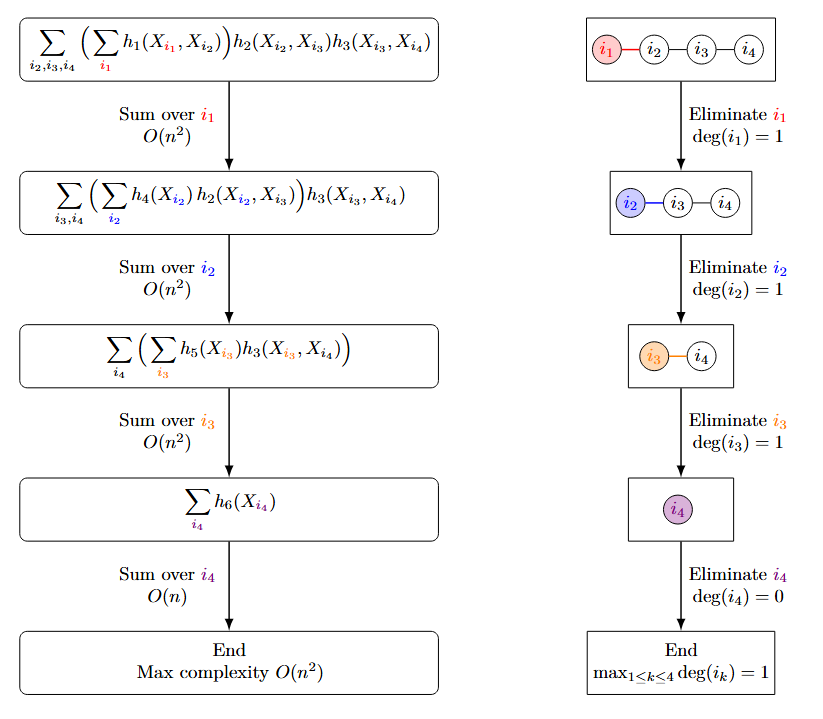
\includegraphics[width=0.8\linewidth]{complexity.jpg}
    \caption*{Procedure of Computing a 4-th order V-statistic with $\calA = ((1,2),(2,3),(3,4))$}
\end{figure}
\end{frame}


\begin{frame}
\frametitle{The Answer  to Question 1: Complexity}
\begin{itemize}
\setlength\itemsep{1.5em}
        \item In general, the computational complexity of a $V$-statistics depends on the summation ordering.
            \vspace{1.5em}
            \begin{itemize}
            \setlength\itemsep{1.5em}
        \item The optimal ordering corresponding to the \textbf{treewidth} of the corresponding graph $G$.
        precisely $O(n^{\operatorname{tw}(G)+1})$. 

                \item Finding the optimal ordering is known to be NP-hard. 
                \item In practice, heuristic algorithm such as greedy algorithm is used.  
                \item In the low-order case, the proof can be derived manually.
        \end{itemize}

\item For $U$-statistics, the computational complexity is determined by the maximum treewidth across all graphical representations induced by the corresponding $V$-statistics.
        
\end{itemize}
    
\end{frame}



\section{Applications}
\begin{frame}
    \frametitle{Outline}
    \tableofcontents[currentsection, sectionstyle=show/shaded, subsectionstyle=show/shaded/shaded]
\end{frame}
\begin{frame}
    \frametitle{Application 1: Higher-Order Influence Functions}
    \begin{itemize}
        \item HOIFs involve computing a class of U-statistics like
              \begin{align*}
                h^{\mathsf{HOIF}}_m(X_{1}, \ldots, X_{m})  = f_1(X_{1},X_{2})  f_2(X_{2},X_{3}) \cdots f_{m-1}(X_{m-1},X_{m})
              \end{align*}
        \item We test \package{} on computing HOIFs on platforms both in CPU and GPU (with \torch).
        \item For CPU
              \begin{table}[htbp]
                  \centering
                  \caption{Average runtime (in seconds) using CPU parallel computation. Experiments were conducted on Intel Xeon ICX Platinum 8358 CPUs (2.6GHz, 64 total cores) with 512 GB of memory, evaluated across varying sample sizes and orders of HOIF-type U-statistics.}
                  \label{tab:HOIF_CPU}
                  \begin{tabular}{cccccc}
                      \toprule
                      $\bm{m} \backslash \bm{n}$ & \textbf{1000} & \textbf{2000} & \textbf{4000} & \textbf{8000} & \textbf{10000} \\
                      \midrule
                      2                          & 0.64          & 0.00141       & 0.01298       & 0.03174       & 0.04746        \\
                      3                          & 0.00396       & 0.01518       & 0.07392       & 0.26849       & 0.45976        \\
                      4                          & 0.02321       & 0.07313       & 0.32765       & 2.09545       & 2.36766        \\
                      5                          & 0.09853       & 0.36239       & 1.71419       & 9.11349       & 14.21350       \\
                      6                          & 0.38878       & 1.47719       & 7.44444       & 40.22143      & 58.85063       \\
                      7                          & 1.91677       & 6.75947       & 34.08805      & 195.31414     & 290.54295      \\
                      \bottomrule
                  \end{tabular}
              \end{table}
    \end{itemize}
\end{frame}

\begin{frame}
    \frametitle{Application 1: Higher-Order Influence Functions}
    \begin{itemize}
        \item For GPU
              \begin{table}[htbp]
                  \centering
                  \caption{Average runtime (in seconds) using a single GPU (NVIDIA RTX 4090, 24GB) with parallel computation, across varying sample sizes and orders of HOIF-type U-statistics.}
                  \label{tab:HOIF_GPU}
                  \begin{tabular}{cccccc}
                      \toprule
                      $\bm{m} \backslash \bm{n}$ & \textbf{1000} & \textbf{2000} & \textbf{4000} & \textbf{8000} & \textbf{10000} \\
                      \midrule
                      2                          & 0.00184       & 0.00151       & 0.00155       & 0.00238       & 0.00339        \\
                      3                          & 0.00172       & 0.00147       & 0.00193       & 0.00577       & 0.00745        \\
                      4                          & 0.00305       & 0.00353       & 0.00707       & 0.03612       & 0.06245        \\
                      5                          & 0.00835       & 0.01089       & 0.03456       & 0.19807       & 0.36160        \\
                      6                          & 0.02608       & 0.03906       & 0.16981       & 1.12072       & 2.13328        \\
                      7                          & 0.12031       & 0.19132       & 0.91884       & 6.45225       & 12.21350       \\
                      \bottomrule
                  \end{tabular}
              \end{table}
    \end{itemize}
\end{frame}

\begin{frame}
    \frametitle{Application 2: Distance Covariance}
    \begin{itemize}
        \item We also test our algorithm on computing $\mathsf{dCov}^2$
              \begin{align*}
                  \mathsf{dCov}^2(X, Y) = \frac{(n-4)!}{n!} \sum_{i \neq j \neq q \neq r}
                  a_{ij}b_{qr} + a_{ij}b_{ij} - a_{ij}b_{iq} - a_{ij}b_{jr}
              \end{align*}
        \item We compare the performance with \cite{shao2025u}, $n =138$.
              \begin{itemize}
                  \item They use a randomized incomplete algorithm to compute $\mathsf{dCov}^2$.
                  \item $\alpha$ is a tuning parameter to control the degree of completeness.
                  \item Randomized algorithm of $\alpha$ takes $O(n^{\alpha})$ time.
              \end{itemize}

    \end{itemize}
\begin{table}[htbp]
\centering
\caption{
Runtime (in seconds) comparison of various methods for computing $\mathsf{dCov}^{2}$. 
Experiments were run on Intel Xeon ICX Platinum 8358 CPUs (2.6GHz, 64 total cores) with memory of 512 GB. 
}
\label{tab:dcov}
\scalebox{0.85}{
\begin{tabular}{cc|cccc}
\toprule
\multicolumn{2}{c|}{\package{}} & \multicolumn{4}{c}{\citet{shao2025u}'s \texttt{MATLAB} code} \\ 
\cmidrule(lr){1-2} \cmidrule(lr){3-6}
\makecell{\textbf{No Parallel}} & 
\makecell{\textbf{Parallel}} & 
\makecell{\textbf{Randomized} \\ $\alpha = 1.5$} &
\makecell{\textbf{Randomized} \\ $\alpha = 2.0$} &  
\makecell{\textbf{Randomized} \\ $\alpha = 2.5$} & 
\makecell{\textbf{Complete}} \\ 
\midrule
4.0928 & 0.1847 & 0.4211 & 4.5744 & 53.0265 & 3395.4001 \\
\bottomrule
\end{tabular}
}
\end{table}

\end{frame}

\begin{frame}
    \frametitle{Application 3: Motif Counts}
    \begin{itemize}
    \setlength\itemsep{1.5em}
        \item We compare the performance of our \package{} with  \igraph{}.
        \item On Erdős-Rényi graphs $G(n, p)$:
            \begin{itemize}
            \setlength\itemsep{1.5em}
                \item $n$ is the number of vertices. 
                \item $p$ is the probability of edge existence. 
                \item CPU parallel with 64 cores via \torch{} for \package{}.
                \item Count all types of 3-node or 4-node motifs. 
            \end{itemize}
    \end{itemize}
\end{frame}

\begin{frame}
    \frametitle{Application 3: Motif Counts}
    \begin{itemize}
        \item For the 3-node motifs,
    \end{itemize}
    \begin{table}
        \centering
        \caption{
            Runtime comparison of exact all $3$-node motif counts using \texttt{u-stats} and \texttt{igraph} on Erdős-Rényi graphs $G(n, p)$ with $n = 5623$.
            Experiments were run on Intel Xeon ICX Platinum 8358 CPUs (2.6GHz, 64 total cores) with 512 GB of memory.
            "Speedup ratio" compares \texttt{igraph} to our parallel method; "single core speedup" assumes single-core execution.
        }
        \label{tab:motif_counts_3}
        \begin{tabular}{ccccc}
            \toprule
            \makecell{\textbf{Edge}                      \\ \textbf{Prob.} $p$} & \makecell{\textbf{\texttt{u-stats}} \\ \textbf{Time (s)}} & \makecell{\textbf{\texttt{igraph}} \\ \textbf{Time (s)}} &\makecell{\textbf{Speedup} \\ \textbf{Ratio}} &  \makecell{\textbf{Single-Core} \\ \textbf{Speedup}} \\
            \midrule
            0.001 & 0.617 & 0.025    & 0.040    & 0.001  \\
            0.005 & 0.649 & 0.353    & 0.544    & 0.008  \\
            0.010 & 0.692 & 1.795    & 2.595    & 0.041  \\
            0.020 & 0.783 & 10.594   & 13.529   & 0.211  \\
            0.050 & 1.038 & 136.272  & 131.288  & 2.051  \\
            0.080 & 1.298 & 514.702  & 396.415  & 6.194  \\
            0.100 & 1.453 & 960.299  & 660.690  & 10.323 \\
            0.150 & 1.864 & 3003.490 & 1611.389 & 25.178 \\
            0.200 & 2.275 & 6725.515 & 2955.656 & 46.182 \\
            \bottomrule
        \end{tabular}
    \end{table}
\end{frame}

\begin{frame}
    \frametitle{Application 3: Motif Counts}

    \begin{itemize}
        \item For the 4-node motifs,
    \end{itemize}
    \begin{table}
        \centering
        \caption{
            Runtime comparison of exact all $4$-node motif counts using \texttt{u-stats} and \texttt{igraph} on Erdős-Rényi graphs $G(n, p)$ with $n = 2000$.
            Experiments were run on Intel Xeon ICX Platinum 8358 CPUs (2.6GHz, 64 total cores) with 512 GB of memory.
            "Speedup ratio" compares \texttt{igraph} to our parallel method; "single core speedup" assumes single-core execution.
        }
        \label{tab:motif_counts_4}
        \begin{tabular}{ccccc}
            \toprule
            \makecell{\textbf{Edge}                       \\ \textbf{Prob.} $p$} & \makecell{\textbf{\texttt{u-stats}} \\ \textbf{Time (s)}} & \makecell{\textbf{\texttt{igraph}} \\ \textbf{Time (s)}} &\makecell{\textbf{Speedup} \\ \textbf{Ratio}} &  \makecell{\textbf{Single-Core} \\ \textbf{Speedup}} \\
            \midrule
            0.001 & 70.959 & 0.004     & 0.      & 0.     \\
            0.005 & 71.947 & 0.168     & 0.002   & 0.     \\
            0.010 & 68.463 & 1.453     & 0.021   & 0.     \\
            0.020 & 65.634 & 15.573    & 0.237   & 0.004  \\
            0.050 & 65.786 & 394.532   & 5.997   & 0.094  \\
            0.080 & 66.866 & 2371.373  & 35.465  & 0.554  \\
            0.100 & 68.219 & 5396.057  & 79.099  & 1.236  \\
            0.150 & 65.969 & 23003.041 & 348.692 & 5.448  \\
            0.200 & 65.259 & 61796.760 & 946.940 & 14.796 \\
            \bottomrule
        \end{tabular}
    \end{table}
\end{frame}

\section{Limitations and Future Work}
\begin{frame}
    \frametitle{Outline}
    \tableofcontents[currentsection, sectionstyle=show/shaded, subsectionstyle=show/shaded/shaded]
\end{frame}
\begin{frame}
    \frametitle{Limitations and Future Work}
    \begin{itemize}
    \setlength\itemsep{1.5em}
        \item Limitations:
              \begin{itemize}
              \setlength\itemsep{1.5em}
                  \item Memory usage is high: for HOIFs, it's not available for sample size larger than $2000$ and order larger than $8$ -- Hybrid between for-loop \& Einsum (or we can wait for better GPUs)?

                  \item How to combine our techniques with randomized incomplete U-statistics \citep{chen2019randomized, shao2025u}?
              \end{itemize}
        \item Future work:
              \begin{itemize}
                  \item Interface for \texttt{R}.
                  \item Non-scalar-valued U-statistics.
              \end{itemize}
    \end{itemize}
\end{frame}

\section*{References}
\begin{frame}
    \frametitle{References}
    \bibliography{Master}
\end{frame}


\begin{frame}
\frametitle{}
    \centering
    \vspace{2cm}
    {\Huge \textbf{Thank You!}} \\[1.5em]

    {\large For more details:} \\[1em]

    \begin{itemize}\setlength\itemsep{0.8em}
        \item Paper draft (arXiv): \\
        \href{https://arxiv.org/abs/2508.12627}{\texttt{https://arxiv.org/abs/2508.12627}}
        
        \item Software (GitHub): \\
        \href{https://github.com/Amedar-Asterisk/U-Statistics-python}{\texttt{github.com/Amedar-Asterisk/U-Statistics-python}}
        
        \item Personal website: \\
        \href{https://cxy0714.github.io/}{\texttt{cxy0714.github.io}}
    \end{itemize}

    \vfill
\end{frame}

\end{document}